\documentclass{article}
\usepackage{preamble}
\begin{document}
\centering

\pgfplotsset{width=240pt, height=150pt}

%%% Plots modeled after https://www.physicsclassroom.com/calcpad/launch/CPK10
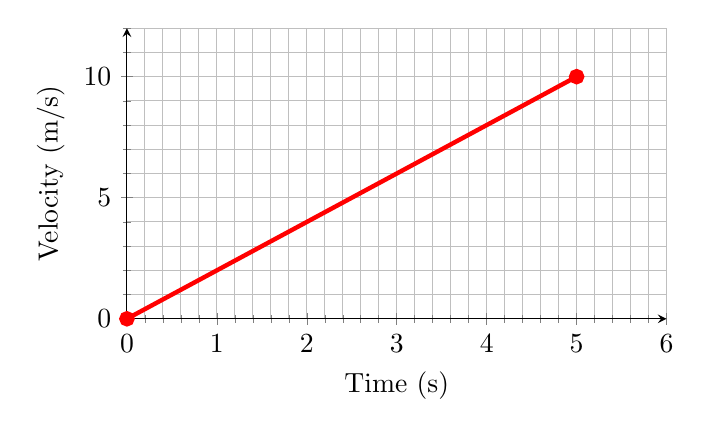
\begin{tikzpicture}
\begin{axis}[width=240pt, height=150pt,
        axis y line=left, 
        axis x line=left,
        ymin=0, ymax=12,
        xmin=0, xmax=6,
        ylabel = Velocity (m/s),
        xlabel = Time (s),
        grid=both,
        ytick={0,5,...,15},
        yminorgrids=true, minor y tick num=4,
        xminorgrids=true, minor x tick num=4,
    ]
    \addplot[
        color=red,
        mark options={color=red},mark=*,
        ultra thick,
        ]
        coordinates {
        (0,0)(5,10)
        };
\end{axis}
\end{tikzpicture} 

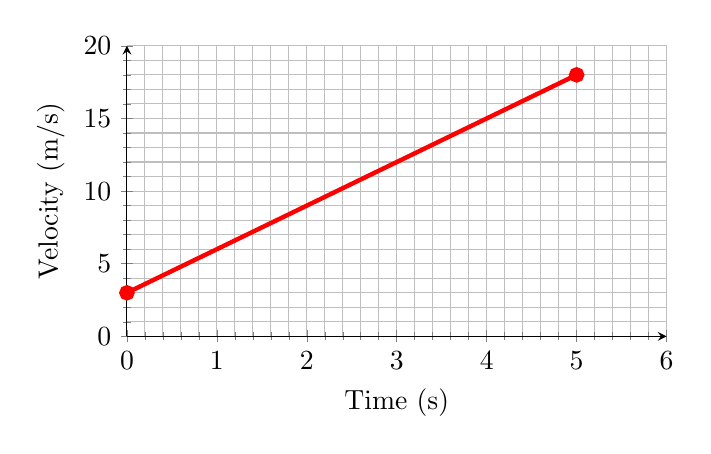
\begin{tikzpicture}
\begin{axis}[width=240pt, height=150pt,
        axis y line=left, 
        axis x line=left,
        ymin=0, ymax=20,
        xmin=0, xmax=6,
        ylabel = Velocity (m/s),
        xlabel = Time (s),
        grid=both,
        ytick={0,5,...,20},
        yminorgrids=true, minor y tick num=4,
        xminorgrids=true, minor x tick num=4,
    ]
    \addplot[
        color=red,
        mark options={color=red},mark=*,
        ultra thick,
        ]
        coordinates {
        (0,3)(5,18)
        };
\end{axis}
\end{tikzpicture} 

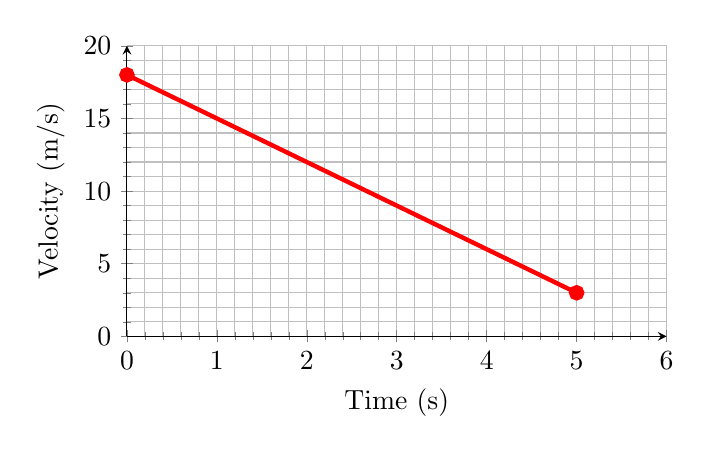
\begin{tikzpicture}
\begin{axis}[width=240pt, height=150pt,
        axis y line=left, 
        axis x line=left,
        ymin=0, ymax=20,
        xmin=0, xmax=6,
        ylabel = Velocity (m/s),
        xlabel = Time (s),
        grid=both,
        ytick={0,5,...,20},
        yminorgrids=true, minor y tick num=4,
        xminorgrids=true, minor x tick num=4,
    ]
    \addplot[
        color=red,
        mark options={color=red},mark=*,
        ultra thick,
        ]
        coordinates {
        (0,18)(5,3)
        };
\end{axis}
\end{tikzpicture} 

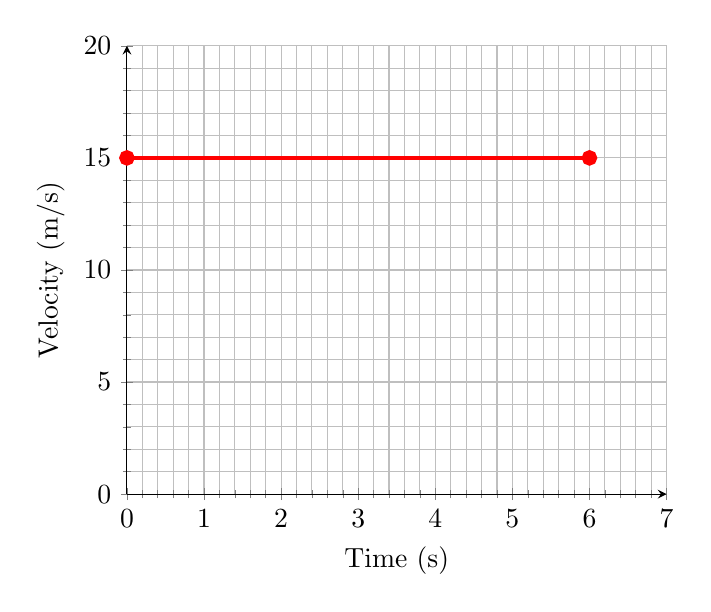
\begin{tikzpicture}
\begin{axis}[axis y line=left, 
        axis x line=left,
        ymin=0, ymax=20,
        xmin=0, xmax=7,
        ylabel = Velocity (m/s),
        xlabel = Time (s),
        grid=both,
        ytick={0,5,...,20},
        % ymajorgrids=true,
        % xmajorgrids=true,
        yminorgrids=true, minor y tick num=4,
        xminorgrids=true, minor x tick num=4,
    ]
    %\fill[black!20] (axis cs: 0,0) rectangle (axis cs: 6,15);
    \addplot[
        color=red,
        mark options={color=red},mark=*,
        ultra thick,
        ]
        coordinates {
        (0,15)(6,15)
        };
\end{axis}
\end{tikzpicture}

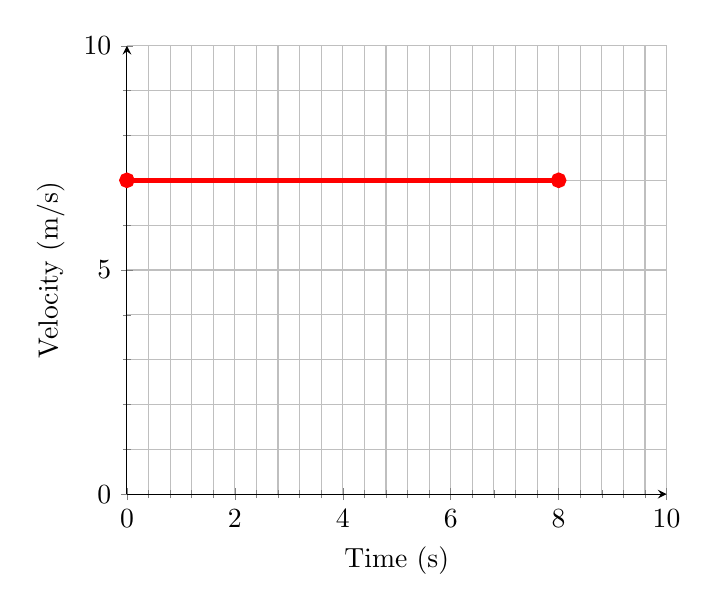
\begin{tikzpicture}
\begin{axis}[axis y line=left, 
        axis x line=left,
        ymin=0, ymax=10,
        xmin=0, xmax=10,
        ylabel = Velocity (m/s),
        xlabel = Time (s),
        grid=both,
        ytick={0,5,...,10},
        % ymajorgrids=true,
        % xmajorgrids=true,
        yminorgrids=true, minor y tick num=4,
        xminorgrids=true, minor x tick num=4,
    ]
    %\fill[black!20] (axis cs: 0,0) rectangle (axis cs: 6,15);
    \addplot[
        color=red,
        mark options={color=red},mark=*,
        ultra thick,
        ]
        coordinates {
        (0,7)(8,7)
        };
\end{axis}
\end{tikzpicture}



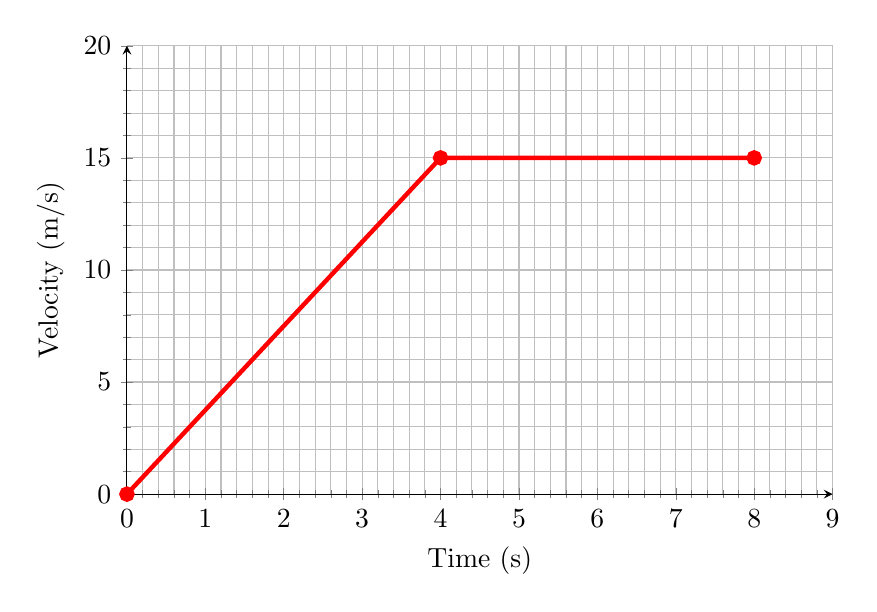
\begin{tikzpicture}
\begin{axis}[width=300pt, height=207pt,
        axis y line=left, 
        axis x line=left,
        ymin=0, ymax=20,
        xmin=0, xmax=9,
        ylabel = Velocity (m/s),
        xlabel = Time (s),
        grid=both,
        ytick={0,5,...,20},
        yminorgrids=true, minor y tick num=4,
        xminorgrids=true, minor x tick num=4,
    ]
    \addplot[
        color=red,
        mark options={color=red},mark=*,
        ultra thick,
        ]
        coordinates {
        (0,0)(4,15)(8,15)
        };
\end{axis}
\end{tikzpicture}

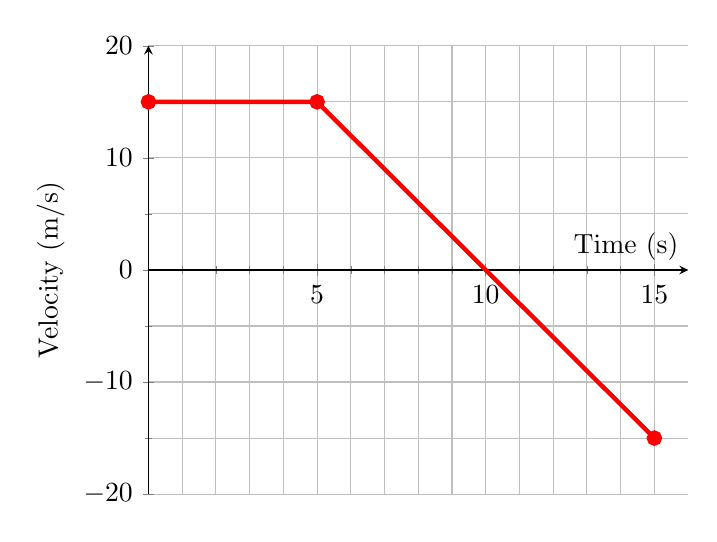
\begin{tikzpicture}
\begin{axis}[
    axis y line=left, 
    axis x line=center,
    xlabel = Time (s),
    ylabel = Velocity (m/s),
    ymin=-20, ymax=20,
    xmin=0, xmax=16,
    ytick={-20,-10,...,20},
    xtick={0,5,...,15},
    ymajorgrids=true,
    xmajorgrids=true,
    yminorgrids=true, minor y tick num=1,
    xminorgrids=true, minor x tick num=4,
    % x label style={anchor=west},
    clip=false,
]
    \addplot[
        %color=green!67!black,
        color=red,
        mark options={color=red},mark=*,
        ultra thick,
        ]
        coordinates {
        (0,15)
        (5,15)
        (15,-15)
        };
\end{axis}
\end{tikzpicture}

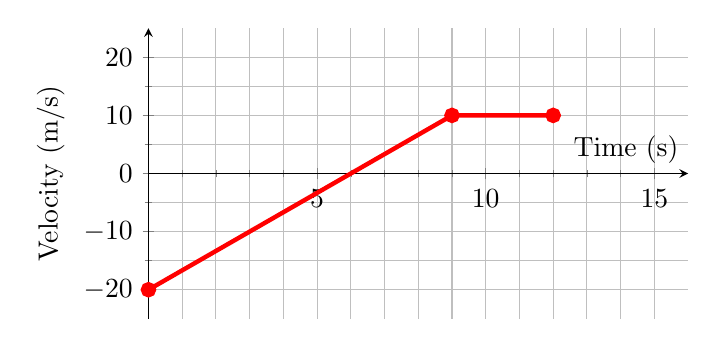
\begin{tikzpicture}
\begin{axis}[width=240pt,height=150pt,
    axis y line=left, 
    axis x line=center,
    xlabel = Time (s),
    ylabel = Velocity (m/s),
    ymin=-25, ymax=25,
    xmin=0, xmax=16,
    ytick={-20,-10,...,20},
    xtick={0,5,...,15},
    ymajorgrids=true,
    xmajorgrids=true,
    yminorgrids=true, minor y tick num=1,
    xminorgrids=true, minor x tick num=4,
    % x label style={anchor=west},
    clip=false,
]
    \addplot[
        %color=green!67!black,
        color=red,
        mark options={color=red},mark=*,
        ultra thick,
        ]
        coordinates {
        (0,-20)
        (9,10)
        (12,10)
        };
\end{axis}
\end{tikzpicture}

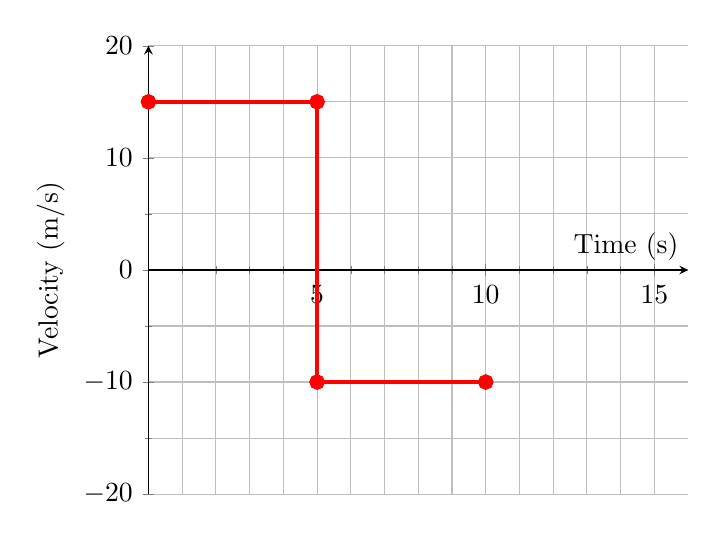
\begin{tikzpicture}
\begin{axis}[
    axis y line=left, 
    axis x line=center,
    xlabel = Time (s),
    ylabel = Velocity (m/s),
    ymin=-20, ymax=20,
    xmin=0, xmax=16,
    ytick={-20,-10,...,20},
    xtick={0,5,...,15},
    ymajorgrids=true,
    xmajorgrids=true,
    yminorgrids=true, minor y tick num=1,
    xminorgrids=true, minor x tick num=4,
    % x label style={anchor=west},
    clip=false,
]
    \addplot[
        %color=green!67!black,
        color=red,
        mark options={color=red},mark=*,
        ultra thick,
        ]
        coordinates {
        (0,15)
        (5,15)
        (5,-10)
        (10,-10)
        };
\end{axis}
\end{tikzpicture}

% \begin{tikzpicture}
%     \begin{axis}[axis y line=left, 
%         axis x line=left,
%         ymin=0, ymax=175,
%         xmin=0, xmax=30,
%         ylabel = Velocity (m/s),
%         xlabel = Time (s),
%         grid=both,
%         ytick={0,25,...,175}
%     ]
%     \addplot[
%         %color=green!67!black,
%         color=black,
%         mark options={color=black},mark=*,
%         ultra thick,
%         ]
%         coordinates {
%         (0,25)(5,50)(10,75)(15,100)(20,125)(25,150)
%         };
%     \end{axis}
%     \end{tikzpicture}
    
% \begin{tikzpicture}
% \begin{axis}[axis y line=left, 
%     axis x line=left,
%     ymin=0, ymax=125,
%     xmin=0, xmax=30,
%     ylabel = Velocity (m/s),
%     xlabel = Time (s),
%     grid=both,
%     ytick={0,25,...,175}
% ]
% \addplot[
%     %color=green!67!black,
%     color=black,
%     mark options={color=black},mark=none,
%     ultra thick,
%     ]
%     coordinates {
%     (0,0)(5,25)(10,50)(15,75)(20,100)(25,100)(30,100)
%     };
% \end{axis}
% \end{tikzpicture}

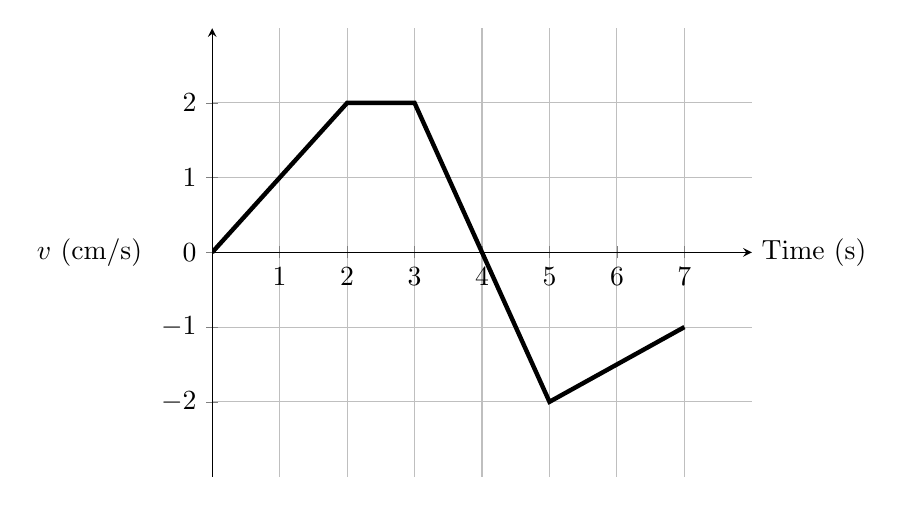
\begin{tikzpicture}
\begin{axis}[
    axis y line=left, 
    axis x line=center,
    every axis x label/.style={at={(current axis.right of origin)},anchor=west},
    xlabel = Time (s),
    ylabel = $v$ (cm/s),
    ylabel style={rotate=-90},
    ymin=-3, ymax=3,
    xmin=0, xmax=8,
    ytick={-2,-1,...,2},
    xtick={0,1,...,7},
    ymajorgrids=true,
    xmajorgrids=true,
]
    \addplot[
        %color=green!67!black,
        color=black,
        mark options={color=black},mark=none,
        ultra thick,
        ]
        coordinates {
        (0,0)(2,2)(3,2)(5,-2)(7,-1)
        };
\end{axis}
\end{tikzpicture}

%     \begin{tikzpicture}
%     \begin{axis}[axis y line=left, 
%         axis x line=left,
%         ymin=0, ymax=12,
%         xmin=0, xmax=10,
%         ylabel = Velocity (yd/s),
%         xlabel = Time (s),
%         grid=both,
%         ytick={0,2,...,12}
%     ]
%     \addplot[
%         %color=green!67!black,
%         color=black,
%         mark options={color=black},mark=none,
%         ultra thick,
%         ]
%         coordinates {
%         (0,4)
%         (4,8)
%         (8,8)
%         };
%     \end{axis}
%     \end{tikzpicture}
    
% \begin{tikzpicture}
%     \begin{axis}[axis y line=left, 
%         axis x line=left,
%         ymin=0, ymax=40,
%         xmin=0, xmax=45,
%         ylabel = Velocity (m/s),
%         xlabel = Time (s),
%         grid=both,
%         ytick={0,10,...,70},
%         xtick={0,5,...,45}
%     ]
%     \addplot[
%         %color=green!67!black,
%         color=black,
%         mark options={color=black},mark=none,
%         ultra thick,
%         ]
%         coordinates {
%         (0,0)
%         (10,30)
%         (20,30)
%         (40,0)
%         };
%     \end{axis}
% \end{tikzpicture}

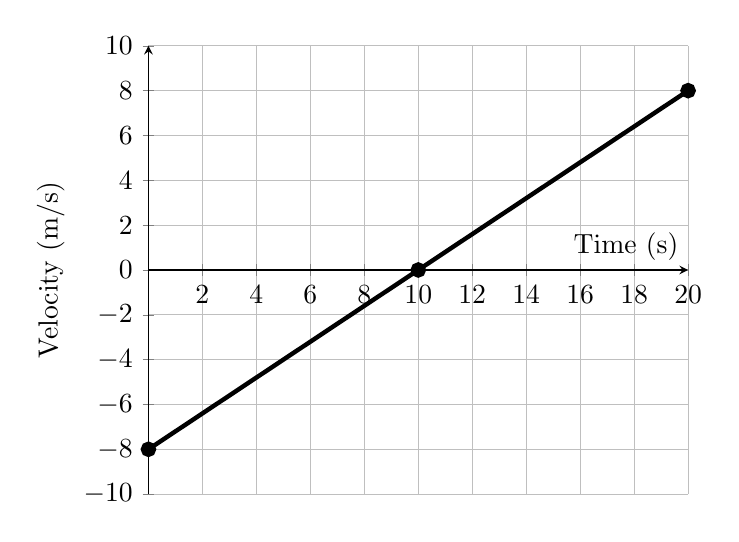
\begin{tikzpicture}
\begin{axis}[
    axis y line=left, 
    axis x line=center,
    xlabel = Time (s),
    ylabel = Velocity (m/s),
    ymin=-10, ymax=10,
    xmin=0, xmax=20,
    ytick={-10,-8,...,10},
    xtick={0,2,...,20},
    ymajorgrids=true,
    xmajorgrids=true,
    % x label style={anchor=west},
    clip=false,
]
    \addplot[
        %color=green!67!black,
        color=black,
        mark options={color=black},mark=*,
        ultra thick,
        ]
        coordinates {
        (0,-8)
        (10,0)
        (20,8)
        };
\end{axis}
\end{tikzpicture}


\end{document}